\section*{Semaphores (yet another synchronization primitive)}
\begin{itemize}
\item semaphore is just an integer value, accompanied by a queue of threads (waiting for signals) and manipulated with 2 routines: \texttt{P()} and \texttt{V()}
\item in POSIX, \texttt{P()} $\to$ \texttt{sem\_wait()}; \texttt{V()} $\to$ \texttt{sem\_post()}; \mo{must first} \texttt{sem\_init()}
\item tweaking init sem vals to impl. locks, cond vars, other conc primitives
\end{itemize}
\begin{lstlisting}[language=c]
#include <semaphore.h> // if pshared == 0: sem shared btw thds in same
int sem_init(sem_t *sem, int pshared, unsigned int value); // process
int sem_wait(sem_t *sem); // wait on a semaphore
int sem_post(sem_t *sem); // signal the waiting threads
\end{lstlisting}
\begin{minipage}{0.6\linewidth}
\begin{lstlisting}[language=c]
int sem_wait(sem_t *s) {
  /* decrement semaphore `s' by one
  wait if semaphore `s' is negative */
} // assume both wait/post exec atomically
int sem_post(sem_t *s) {
  /* increment semaphore `s' by one
  if waiting threads >= 1, wake one */
}
\end{lstlisting}
\end{minipage}
\begin{minipage}{0.4\linewidth}
\begin{lstlisting}[language=c,xleftmargin=2pt,xrightmargin=2pt]
sem_t m;
// init to X;
// X should be 1 at first
sem_init(&m, 0, X);
/* used as a lock */
sem_wait(&m);
// critical section here
sem_post(&m);
\end{lstlisting}
\end{minipage}
\section*{Binary Semaphores (Locks, code at above right)}
For $N > 1$ threads, the 1st thread to execute \texttt{sem\_wait()}
immediately brings \texttt{s} to 0; other threads will be forced to wait\\
\begin{minipage}{.48\linewidth}
\begin{tabular}[th]{lll}
  \hline
  \multicolumn{3}{l}{trace single T using a sem}\\
  \textbf{sem} & $T_0$ & $T_1$\\
  \hline
  1 & & \\
  1 & call \texttt{sem\_wait()} & \\
  0 & \texttt{sem\_wait()} returns & \\
  0 & (\texttt{crit sect}) & \\
  0 & call \texttt{sem\_post()} & \\
  1 & \texttt{sem\_post()} returns\\
  \hline
\end{tabular}
\end{minipage}
\begin{minipage}{.52\linewidth}
  \flushleft
  \begin{itemize}
  \item $T_0$ calls \texttt{sem\_wait()}, dec \texttt{sem}: $1 \to 0$
  \item then $T_0$ will wait only if sem $\leq$ 0
  \item $\because$ \texttt{sem == 0} now, \texttt{sem\_wait()} will simply return and $T_0$ will continue
  \item $T_0$ now free to enter critical sect.
  \item If no other thd tries to acquire lock while $T_0$ in critical sect, when $T_0$ calls \texttt{sem\_post()}, it will restore \texttt{sem} ($0 \to 1$) and wake no waiting thread, $\because$ there are none
  \end{itemize}
\end{minipage}
Run (running); Ready (runnable not running); Sleep (thread is blocked)
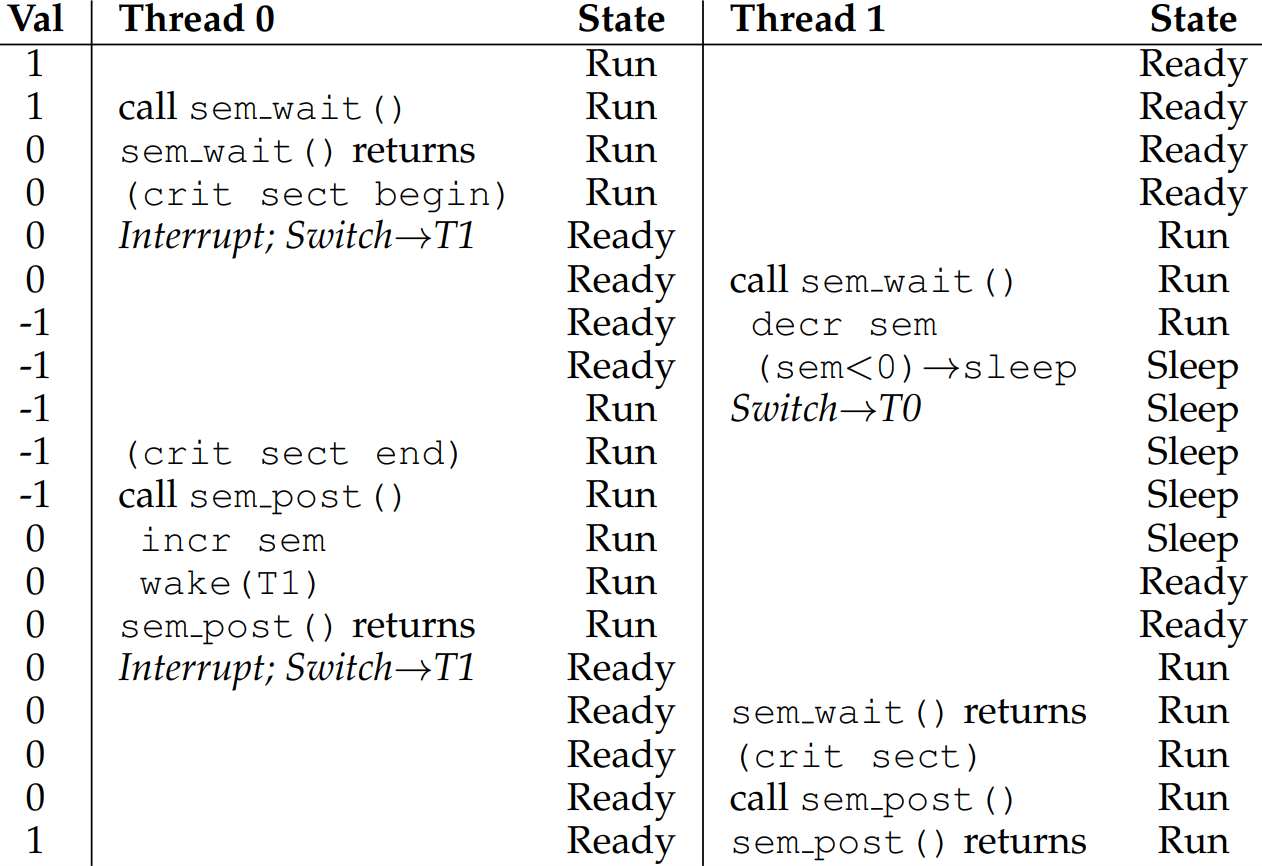
\includegraphics[width=\linewidth,height=6cm]{imgs/twots_usesem2}
\section*{Semaphores for ordering events in concurrent programs}
\begin{minipage}{.4\linewidth}
\begin{lstlisting}[language=c,xleftmargin=2pt,xrightmargin=2pt]
sem_t s; // expected:
/* parent: begin
   child
   parent: end */
void *child(void *arg) {
  printf("child\n");
  sem_post(&s); // signal
  return NULL;
}
\end{lstlisting}
\end{minipage}
\begin{minipage}{.6\linewidth}
\begin{lstlisting}[language=c,xleftmargin=2pt,xrightmargin=2pt]
int main(int argc, char *argv[]) {
  sem_init(&s, 0, X); // X should be 0
  printf("parent: begin\n");
  pthread_t c;
  pthread_create(&c, NULL, child, NULL);
  sem_wait(&s); // wait here for child
  printf("parent: end\n");
  return 0;
} // simulate pthread_join()
\end{lstlisting}
\end{minipage}
% needed this empty line

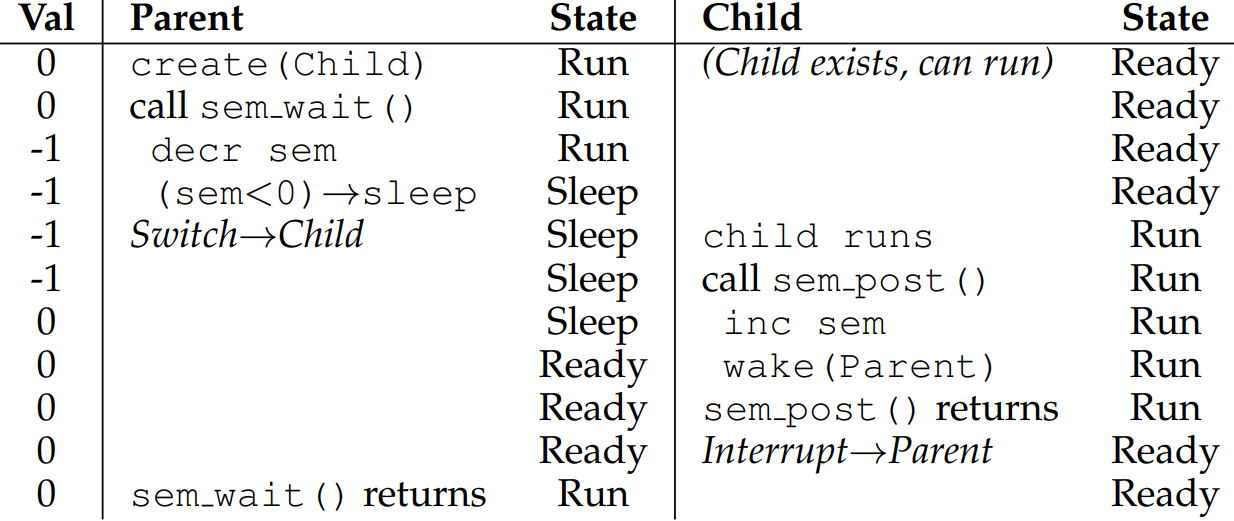
\includegraphics[width=\linewidth,height=4cm]{imgs/pwaitschd}
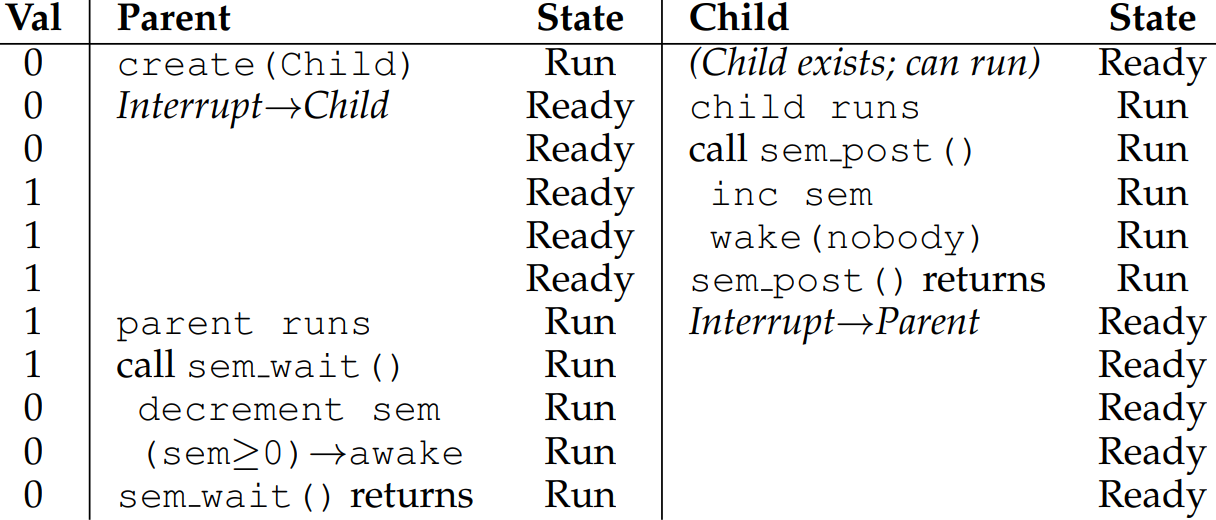
\includegraphics[width=\linewidth,height=4cm]{imgs/chdwaitsp}
\begin{minipage}{.5\linewidth}
\begin{lstlisting}[language=c,xleftmargin=2pt,xrightmargin=2pt]
int buffer[MAX]; // assume MAX = 1
int fill = 0;
int use = 0;
int main(int argc, char *argv[]) {
  // ... init empty = MAX
  sem_init(&empty, 0, MAX);
  sem_init(&full, 0, 0);
  // ... init full = 0
} // assume running on 1 CPU
\end{lstlisting}
\end{minipage}
\begin{minipage}{.5\linewidth}
\begin{lstlisting}[language=c,xleftmargin=2pt,xrightmargin=2pt]
void put(int value) {
  buffer[fill] = value;       // L F1
  fill = (fill + 1) % MAX; // L F2
} // put/get works only if MAX = 1
int get() {
  int tmp = buffer[use]; // L G1
  use = (use + 1) % MAX; // L G2
  return tmp;
}
\end{lstlisting}
\end{minipage}
\begin{minipage}{.5\linewidth}
\begin{lstlisting}[language=c,xleftmargin=2pt,xrightmargin=2pt]
sem_t empty; sem_t full;
void *producer(void *arg) {
  int i;
  for (i = 0; i < loops; i++) {
    sem_wait(&empty); // Line P1
    put(i);             // Line P2
    sem_post(&full);    // Line P3
  }// 2. producer runs & puts P1-2
}  // 3. signals P3 or waits P3-P1
\end{lstlisting}
\end{minipage}
\begin{minipage}{.5\linewidth}
\begin{lstlisting}[language=c,xleftmargin=2pt,xrightmargin=2pt]
void *consumer(void *arg) {
  int tmp = 0;
  while (tmp != -1) {
    sem_wait(&full);    // Line C1
    tmp = get();        // Line C2
    sem_post(&empty);  // Line C3
    printf("%d\n", tmp);
  }// 1. consumer runs & waits C1
}  // 4. wake/take C1-C3 & post C3
\end{lstlisting}
\end{minipage}
\begin{minipage}{.5\linewidth}
\begin{lstlisting}[language=c,xleftmargin=2pt,xrightmargin=2pt,framexbottommargin=2pt]
void *producer(void *arg) {
  int i;
  for (i = 0; i < loops; i++) {
+   sem_wait(&mutex); // Line P0
    sem_wait(&empty); // Line P1
    put(i);             // Line P2
    sem_post(&full);  // Line P3
+   sem_post(&mutex); // Line P4
  }// 3. producer now runs P0
}  // 4. lock held -> deadlock
void *consumer(void *arg) {
  int i;
  for (i = 0; i < loops; i++) {
+   sem_wait(&mutex); // Line C0
    sem_wait(&full);   // Line C1
    int tmp = get();   // Line C2
    sem_post(&empty); // Line C3
+   sem_post(&mutex); // Line C4
    printf("%d\n", tmp);
  }// 1. consumer runs first C0-C1
}  // 2. holds lock and sleeps
\end{lstlisting}
\end{minipage}
\begin{minipage}{.5\linewidth}
\begin{lstlisting}[language=c,xleftmargin=4pt,xrightmargin=0pt,framexbottommargin=2pt]
void *producer(void *arg) {
  int i;
  for (i = 0; i < loops; i++) {
+   sem_wait(&empty); // Line P1
+   sem_wait(&mutex); // Line P1.5
    put(i);             // Line P2
+   sem_post(&mutex); // Line P2.5
+   sem_post(&full);   // Line P3
  }// 2. prod runs & locks P1-P2
}  // 3. puts & unlocks P2-P2.5
void *consumer(void *arg) {
  int i;
  for (i = 0; i < loops; i++) {
+   sem_wait(&full);   // Line C1
+   sem_wait(&mutex); // Line C1.5
    int tmp = get();   // Line C2
+   sem_post(&mutex); // Line C2.5
+   sem_post(&empty); // Line C3
    printf("%d\n", tmp);
  }// 1. consumer runs & sleeps C1
}  // 4. wake,lck,get,unlck C1-2.5
\end{lstlisting}
\end{minipage}
\begin{minipage}{.64\linewidth}
\begin{lstlisting}[language=c,framexbottommargin=1pt]
typedef struct _rwlock_t {
  sem_t lock;        // binary sem (basic lock)
  sem_t writelock; // allow 1 wtr/many rdrs
  int readers;       // #rdrs in critical sect
} rwlock_t;          //reader-writer lock
void rwlock_init(rwlock_t *rw) {
  rw->readers = 0;
  sem_init(&rw->lock, 0, 1);
  sem_init(&rw->writelock, 0, 1);
}
void rwlock_acquire_readlock(rwlock_t *rw) {
  sem_wait(&rw->lock);
  rw->readers++;
  if (rw->readers == 1) // 1st rdr gets wlock
     sem_wait(&rw->writelock);
  sem_post(&rw->lock);
}
void rwlock_release_readlock(rwlock_t *rw) {
  sem_wait(&rw->lock);
  rw->readers--;
  if (rw->readers == 0) // last rdr frees it
     sem_post(&rw->writelock);
  sem_post(&rw->lock);
}
void rwlock_acquire_writelock(rwlock_t *rw) {
  sem_wait(&rw->writelock);
}
void rwlock_release_writelock(rwlock_t *rw) {
  sem_post(&rw->writelock);
}
\end{lstlisting}
\end{minipage}
\begin{minipage}{.37\linewidth}
  \flushleft
  \begin{itemize}
  \item call \texttt{acquire\_wlock()} and \texttt{release\_wlock()} for updating data
  \item \texttt{wlock} sem ensures only a single $T$ acquires lock and enters critical sect
  \item first reader also acquires \texttt{wlock} for more subsequent readers to acquire \texttt{rlock}
  \item any $T_w$ must wait until \mr{all} readers done
  \item last $T_r$ frees \texttt{wlock} and \texttt{rlock}, then exits
  \item readers may starve writers easily in this way
  \end{itemize}
\begin{lstlisting}[language=c,xleftmargin=4pt,xrightmargin=3pt]
while (1) {// dinning ps
  think();
  get_forks(p);
  eat();
  put_forks(p);
}
// two helper fns
int left(int p) {
  return p; }
int right(int p) {
  return (p + 1) % 5; }
\end{lstlisting}
\end{minipage}
\begin{minipage}{.5\linewidth}
\begin{lstlisting}[language=c,xrightmargin=2pt]
sem t forks[5]; // assume init-ed
void get_forks(int p) {
  sem_wait(&forks[left(p)]);
  sem_wait(&forks[right(p)]);
}// if each p gets their left fork
void put_forks(int p) {
  sem_post(&forks[left(p)]);
  sem_post(&forks[right(p)]);
}// all wait for right -> deadlock
\end{lstlisting}
\end{minipage}
\begin{minipage}{.5\linewidth}
\begin{lstlisting}[language=c,xleftmargin=4pt]
void get_forks(int p) {
  if (p == 4) { // p4 & p0 pick f0
    sem_wait(&forks[right(p)]);
    sem_wait(&forks[left(p)]);
  } else { // others pick left
    sem_wait(&forks[left(p)]);
    sem_wait(&forks[right(p)]);
  } // one p will pick two forks
}   // circular dependency broken
\end{lstlisting}
\end{minipage}
\section*{Implement Zemaphores With Locks And Cond Vars}
\begin{minipage}{.5\linewidth}
\begin{lstlisting}[language=c,xrightmargin=2pt]
typedef struct __Zem_t {
  int value;
  pthread_cond_t cond;
  pthread_mutex_t lock;
} Zem_t;
// zem never < 0 in this impl
// only one thread can call this
void Zem_init(Zem_t *s, int value)
{
  s->value = value;
  Cond_init(&s->cond);
  Mutex_init(&s->lock);
}
\end{lstlisting}
\end{minipage}
\begin{minipage}{.5\linewidth}
\begin{lstlisting}[language=c,xleftmargin=4pt]
void Zem_wait(Zem_t *s) {
  Mutex_lock(&s->lock);
  while (s->value <= 0)
    Cond_wait(&s->cond, &s->lock);
  s->value--;
  Mutex_unlock(&s->lock);
}
void Zem_post(Zem_t *s) {
  Mutex_lock(&s->lock);
  s->value++;
  Cond_signal(&s->cond);
  Mutex_unlock(&s->lock);
}
\end{lstlisting}
\end{minipage}
\begin{tcolorbox}[left=0mm, top=1mm, right=0mm, rightlower=0mm, bottom=1mm,
  title=Setting the value of a semaphore,
  halign title=center]
  Consider \# resrc you are willing to give away immediately after init. With lock, it is 1, $\because$ you will have the lock locked (given away) immediately after init. In ordering case, it is 0, $\because$ there's nothing to give away at start; only when child done is the resrc created (inc to 1)
  \tcblower
One good idea may be made slightly broader and thus solve a larger class of problems. However, be careful when generalizing; as Lampson warns us ``Don't generalize; generalizations are generally wrong''.
\end{tcolorbox}
